%Relasjonsalgebra
\chapter{Method}
\section{Parser construction}
Writing a parser from scratch was ruled out early for being too time consuming.
Instead it was decided to use tools for compiler and parser construction to
generate a parser from the XQuery 1.0 and XPath 2.0 grammar specifications
developed by the W3C.

\section{Evaluated alternatives}
\subsection{JFlex/CUP}
JFlex and CUP is a versatile combination consisting of JFlex which is a lexer
generator, and CUP which is a parser generator. These tools can be interfaced to
generate a complete parser with a separate lexical analyzer.

JFlex and CUP produces only LALR parsers, and since the W3C has specified an
LL(1) grammar for XQuery 1.0 and XPath 2.0, the combination of JFlex and CUP was
rejected from this project.

\subsection{JavaCC}
JavaCC could have been a viable alternative as it produces LL(k) parsers,
however compared to Antlr its grammar specification syntax deviated so much
from the W3C EBNF syntax, that grammar would have had to be extensively
rewritten.

\subsection{Antlr}
Antlr is a renowned tool for parser generation, and can generate LL(k) parsers.
Additionally, Antlr accepts a grammar specification syntactically very close to
the EBNF used by the W3C. This is the parser generater chosen for our project,
based on the criteria outlined in this section.

\section{Limitations in Antlr}
\subsection{Unicode}
It is important to note, however, that Antlr has limited support for unicode.
In this project this implies that our parser will not accept unicode characters
in the range from and above 0x10000. This will exclude the supplementary
multilingual plane (SMP) range of unicode characters, as well as the
supplementary ideographic plane (SIP) and the supplementary special-purpose
plane (SSP). These are seldomly used, but this is an important limitation
nonetheless. The Antlr developers have indicated that support for this unicode
range will be added in future versions of Antlr.

As a remedy for this situation it is possible to couple an external lexer with
Antlr which will accept unicode characters in the above mentioned character
ranges. For the sake of simplicity this has not been further investigated nor
implemented in this project.

\section{Rewriting the grammar for Antlr syntax conformity}
\subsection{Lexer vs. parser syntax}
The Antlr parser generator can generate parsers and lexers from a single grammar
file. The distinction between terminals and non-terminals is simply a matter of
convention, where terminals are assumed to start with uppercase letters, and
non-terminals are assumed to start with lowercase letters.

In the grammar specified by the W3C, all the productions (terminals and
non-terminals) all start with uppercase letters. Initially this caused some
confusion, because this grammar naturally generated a very big lexer and a very
small and non-functional parser.

This was mitigated by converting non-terminal productions to start with
lowercase letters.

\subsection{Rewriting the W3C 'dash' operator}
In their specification, the W3c uses a dash operator, which has the following
semantic meaning in a grammar (from \cite{w3c03}, section 6):
\begin{quote}
A - B: matches any string that matches A but does not match B.
\end{quote}
This operator is not supported in Antlr, so it was necessary to rewrite
these productions using \emph{semantic predicates} where necessary. Thankfully,
in the original specification, the usage of the dash operator was rather sparse
and only used in trivial productions.

An example of rewriting the dash operator using semantic predicates:
\begin{verbatim}
// Original production
piTarget : Name - (('X' | 'x') ('M' | 'm') ('L' | 'l'));

// Rewritten production using a semantic predicate
piTarget : n=Name { !$n.getText().equalsIgnoreCase("XML") }?;
\end{verbatim}
The original production can be interpreted as ``piTarget can be a Name, but not
`XML', regardless of character casing''. The syntactic predicate will imitate
this behaviour using the method equalsIgnoreCase(). As can be seen from this
example, a semantic predicate is simply any kind of boolean Java expression.
This is a flexible solution, because the boolean expression can be wrapped in a
method with boolean return type, which for example then can be placed inside a
@members { } clause in the grammar file, or even as a static method in an
external class. This makes it possible to add complex grammar logic without
disturbing grammar brevity, if necessary.

\subsection{Grammar LL(1) conformity}
The grammar specification given by W3C is in a very compact and non-verbose
form, annoted with links to certain constraints and issues that need to be kept
in mind by anyone seeking to write a parser for XQuery and XPath. Here we will
list these constraints and briefly explain their implications for the parser.

\begin{itemize}
  \item 
\end{itemize}

\subsection{Reserved keywords}
A particular feature in XQuery is the lack of reserved keywords. This creates a
series of problems when a lexer based on the verbatim grammar specification from
the W3C is trying to recognize tokens. The culprit is the ambiguously defined
terminal symbols. Some of the base character tokens intersect with each other
and makes it hard if not impossible for the lexer to distinguish two different
tokens composed of different token fragments with intersecting characters.

One possible solution to this problem was to eliminate ambiguities in the lexer.
This approach was tried by finding and removing duplicate characters from token
fragments, and then generalizing the tokens and adding semantic predicates to
check for illegal and/or missing characters.

TODO: example

TODO: result (also note in conclusion)

\subsection{Nested comments}
XQuery allows nested comments, for example:
\begin{verbatim}
(: this is a comment (: this comment is nested :) :)
\end{verbatim}
This is a classic problem in compiler construction, however it can be solved
using standard Antlr syntax, without resorting to custom functions/methods for
consuming input and keeping track of nesting. The original EBNF as specified by
W3C is as follows:
\begin{verbatim}
Comment ::= "(:" (CommentContents | Comment)* ":)"
\end{verbatim}
At first glance, this seems uncomplicated and straight forward, but this grammar
needs to be rewritten to be accepted by an LL(1) parser. A suggestion for a 
solution to this problem was initially found on the Antlr mailing
list\footnote{http://www.antlr.org:8080/pipermail/antlr-interest/2005-July/012967.html},
and we based our implementation on such an approach. This lexer rule will
correctly detect and allow nested comments, and hide them from the parser:
\begin{verbatim}	
Comment : LXQCOMMENTSi 
          (Comment | (COLONSi ~RPARSi)=>COLONSi 
          | (LPARSi ~COLONSi)=>LPARSi 
          | ~(LPARSi | COLONSi | IkkeChar))* 
          RXQCOMMENTSi {$channel=HIDDEN;};
\end{verbatim}
TODO: oppdater eksempelet over (IkkeChar)


\section{Unit testing the grammar}
Unit testing can be a powerful tool for asserting functionality and can be a
helpful aid in debugging and prevention of regression errors.  For unit testing the
grammar specification, gUnit \cite{gunit00} was employed. This tool uses a
syntax similar to Antlr itself, however instead of defining productions, one
defines a set of inputs for some rule, as well as the expected result. Consider
this example:

\begin{verbatim}
gunit XQFT;
@header{package no.ntnu.xqft.parse;}

piTarget: // Test piTarget rule

    // Any case permutation of 'XML' must fail
    "Xml" FAIL
    "XMl" FAIL
    "XML" FAIL
    "XmL" FAIL
\end{verbatim}

This is a complete input file for gUnit, and will automatically discover the
classes XQFTLexer and XQFTParser in the package no.ntnu.xqft.parse. gUnit will
then proceed to invoke the lexer with ``Xml'', ``XMl'', ``XML'', and ``XmL'' as
input, and pass the lexer to an instance of XQFTParser and execute the production
piTarget. For all these inputs, it will assert that the parser emits an error
(i.e it must fail to pass the test).

In case of a test where the parser should not fail, the syntax is as follows:
\begin{verbatim}
forClause:
	"for $a in document(\"abc.xml\")/a/b/text()" OK
\end{verbatim}
Here gUnit will assert that the parser will not fail for the given inpu (i.e it
must not fail to pass the test).

gUnit is also capable of parsing abstract syntax trees built by the generated
parser, but this feature has not been used in this project.

\section{Debugging}
There are several approaches to debugging. Antlrworks \cite{antlrwrks00} is a
simple tool for writing, testing and debugging Antlr grammars. The debugging
interface is useful in that it draws a realtime step-by-step parse tree as the
input is being parsed, as well as displaying a list of parser events.

\section{Scoping and symbol tables}
Scoping was implemented using a simple tree structure consisting of parent- and
child scopes. XQuery only allows new scopes to be defined through the
enclosedExpr production rule. This makes it trivial to start a new scope at the
beginning of a enclosedExpr, and end the scope and the end of an enclosedExpr.
This has been implemented as follows:
\begin{figure}[!h]
\begin{verbatim}
enclosedExpr : 
    LBRACESi {
        Scope parent = this.currentScope; 
        this.currentScope = new Scope(); 
        this.currentScope.setParent(parent); 
    }
    expr 
    RBRACSi { 
        this.currentScope = this.currentScope.getParent(); 
    }
;
\end{verbatim}
\caption{Scoping logic embedded in grammar definition}
\end{figure}

Where this.currentScope is a reference to the ``current'' scope in this
context. This member variable is initiated with an empty scope when an object
of the parser class is instantiated.

The implementation above (which is formatted slightly for brevity) will
automatically build a scope tree as the input is parsed.

The currentScope object, which is an object of type Scope, holds one reference
to a symbol table. The symbol table, which is a simple subclass of
java.util.HashMap, is not capable of performing symbol lookups throughout the
scope tree. This functionality is rather provided by the Scope class. This UML diagram
illustrates the relationship between the Scope, SymTab, and Symbol classes:
\begin{figure}[!h]
  \centering
    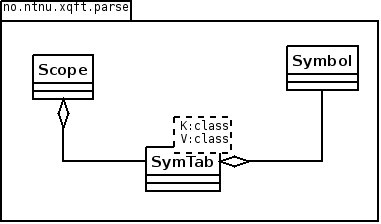
\includegraphics[scale=0.8]{img/uml1}
  \caption{Simplified UML overview of classes related to scope and symbol table}
\end{figure}

\section{Type checking}
XQuery/XPath has a well-defined type hierarchy:
\begin{figure}[!h]
  \centering
    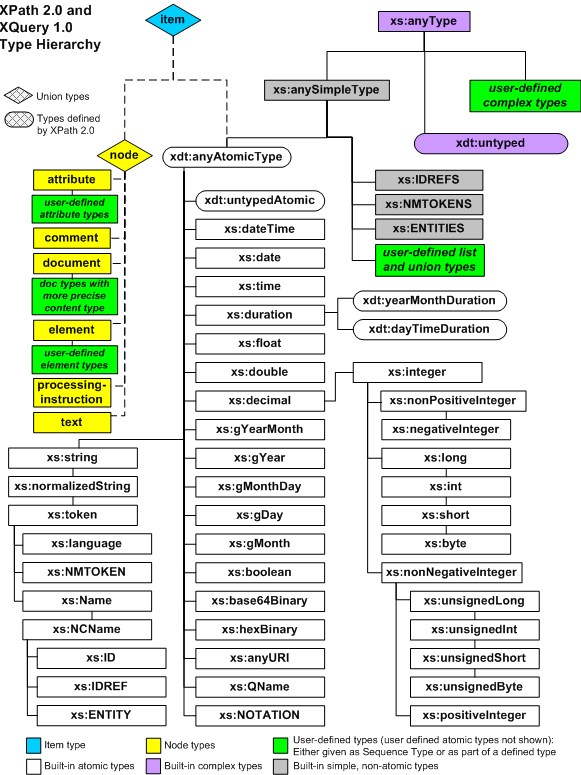
\includegraphics[scale=0.5]{img/xpathtypehierarchy}
  \caption{XQuery/XPath type hierarchy \cite{w3c04} (graphic copyright
  \copyright W3C)}
\end{figure}
All types are derived from the following ``super types'' in the hierarchy:
\begin{itemize}
  \item Node types
  \item Structure types
  \item Atomic types
  \item Simple types
\end{itemize}
There are various implementations of the XQuery